
\documentclass[a4paper,12pt]{article}

\usepackage{minted}
\usepackage[margin=1.2in]{geometry}
\usepackage{enumitem}
\usepackage{graphicx}
\setlength\parindent{0pt}

%opening
\title{Name Sayer User Manual}
\author{By Kungeng Wu and Harrison Leach}

\begin{document}
	
\maketitle
\newpage

\tableofcontents
\cleardoublepage

\listoffigures
\newpage

\section{First Time Launch}
Thank you for using NameSayer for your preferred pronunciation aid. Note that this application is targeted toward student users. 
\\

Before starting Name Sayer, be aware that it will only work on Linux operating systems. Also, note that Java and ffmpeg are required to run the application. 
\\

If you have not already installed these you can do so by typing the following commands into the terminal:
\begin{minted}{bash}
$ sudo apt install default-jre
\end{minted}
\begin{minted}{bash}
$ sudo apt install ffmpeg
\end{minted}

Note that you should also have a database of name recording files ready for use with the application. The application will default to using a database called 'names' (if it exists) in the same directory as the jar. However, you can select your own database from the application. See sections ‘Choose Database’ and ‘How should my database files be named?’ for more information. 
\\

You should also make sure the UserManual.pdf is located in the same directory as the jar file.
\\

To run the application, navigate to the same directory as the jar file and type the following command into the terminal:
\begin{minted}{bash}
$ java -jar NameSayer.jar
\end{minted}
\newpage

\section{Start Menu}
\begin{figure}[!h]
	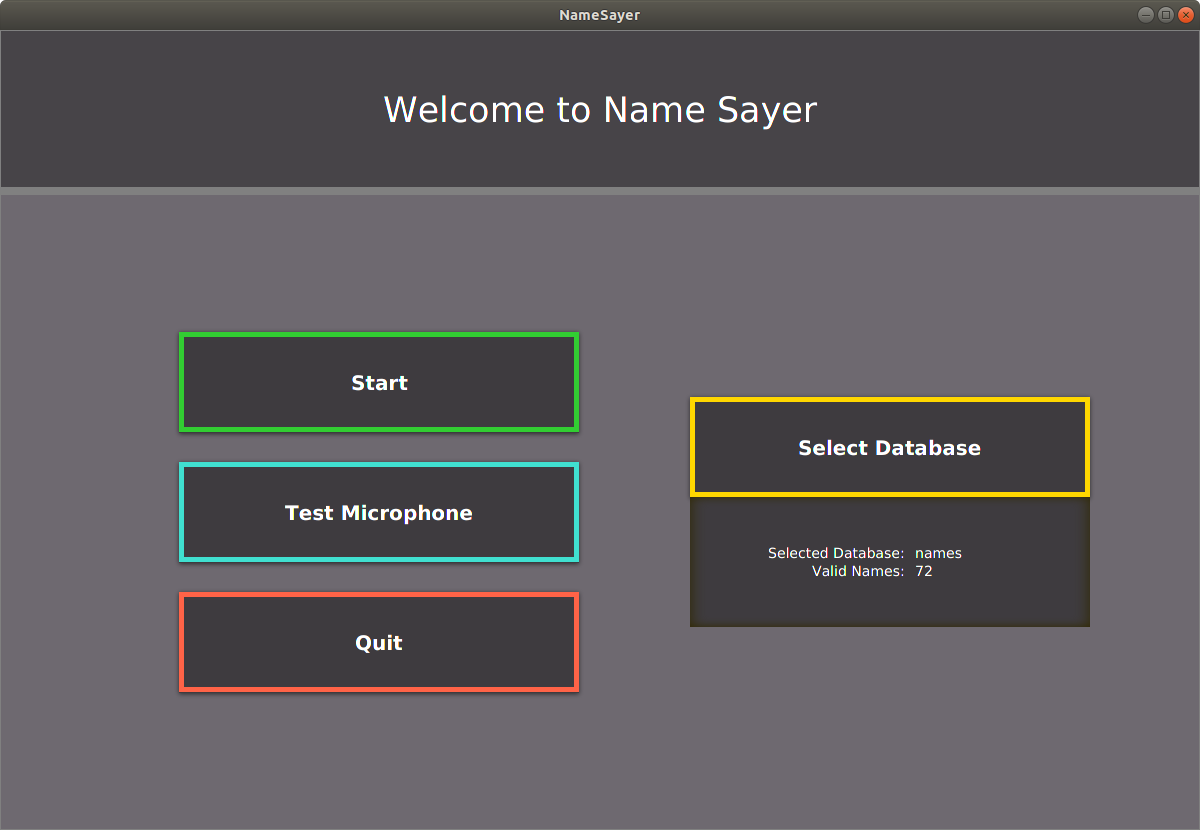
\includegraphics[width=\linewidth]{startmenu.png}
	\caption{Start Menu}
\end{figure}

The entry point of the NameSayer application is the Start Menu (shown in figure 1 above) which allows for microphone checking and database selection before the application is started.

\newpage
\subsection{Test Mic}
\begin{figure}[!h]
	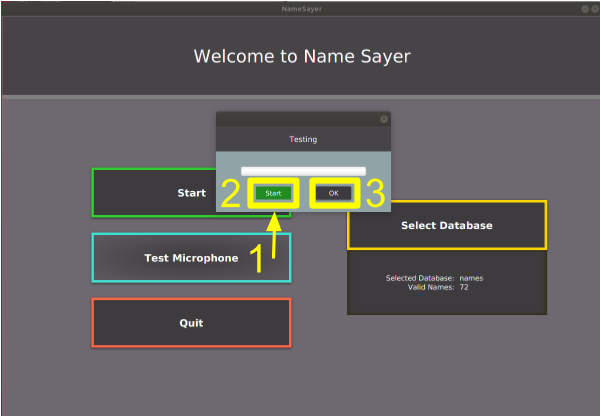
\includegraphics[width=\linewidth]{testmic.png}
	\caption{Test Mic Scene}
\end{figure}
\begin{enumerate}[label=\textbf{\arabic*}]
	\item To test your microphone before starting, press the "Test Microphone" button of the Start Menu. The Testing window will then appear.
	\\
	
	\item Press the "Start" button in the testing window. The bar will now indicate to you the volume of the input received from your microphone. Speak into your microphone to test if it is working.
	\\
	
	\item When you are done testing your microphone, press the "OK" button to close the testing window.
	\\
	
\end{enumerate}
\newpage
\subsection{Select Database} 
\begin{figure}[!h]
	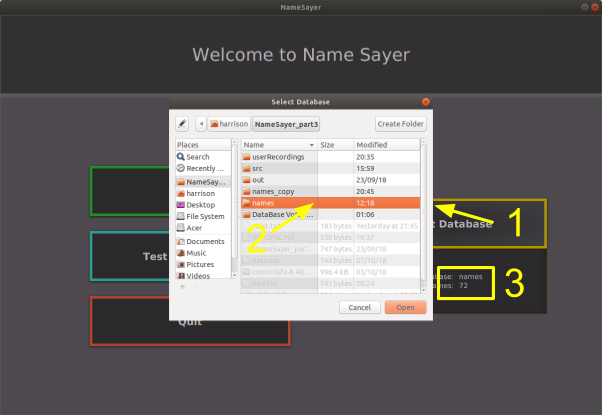
\includegraphics[width=\linewidth]{selectdb.png}
	\caption{Select Database}
\end{figure}
Initially, the default directory used as the database to practise from is called 'names'. This will be empty if the 'names' directory is not in the same directory as the application. If you wish to change the directory that is used for practising you can do so by doing the following:
\\
\begin{enumerate}[label=\textbf{\arabic*}]
	\item Press the "Select Database" button. A window will appear allowing you to choose a directory.
	\\
	
	\item Once you have found the directory you want to select as the database, double-click it or select it and press the "Open" button". The chooser window will close.
	\\
	
	\item Under the "Select Database" button you will be able to confirm you have selected the correct database and you will be able to see how many valid unique names were found from the files in the directory.
	\\
\end{enumerate}
\newpage
\subsection{How should my database files be named?}
 
\begin{figure}[!h]
	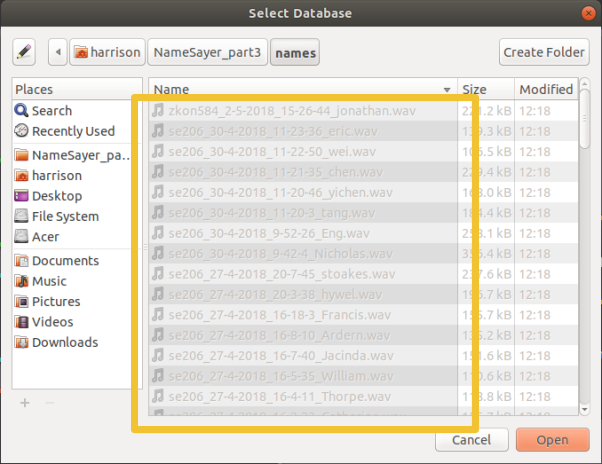
\includegraphics[width=\linewidth]{dbnames.png}
	\caption{Database File Naming}
\end{figure}

The figure above shows an example of the recording files you should be expecting to see inside a database directory. 
\\


In order for recording files to be recognised as a valid name recording file they should have the following file name format:
\\


\textit{$\langle created by\rangle$\_dd-MM-yyyy\_HH-mm-ss\_$\langle name\rangle$.wav}
\\


For example:
\\


\textit{se206\_2-5-2018\_15-23-50\_Mason.wav}
\\


This indicates the recording was created by the se206 class on the 2nd of May 2018 at 3:23:50 PM and the recording is of the Name ‘Mason’.
\\


Recording files MUST be in this format and be a .wav file to be a valid name recording that can be practised by the user.
\newpage
\section{Main Pane}
When you have finished checking your microphone and selected your database, pressing the “Start” button will take you to the Main pane.

\begin{figure}[!h]
	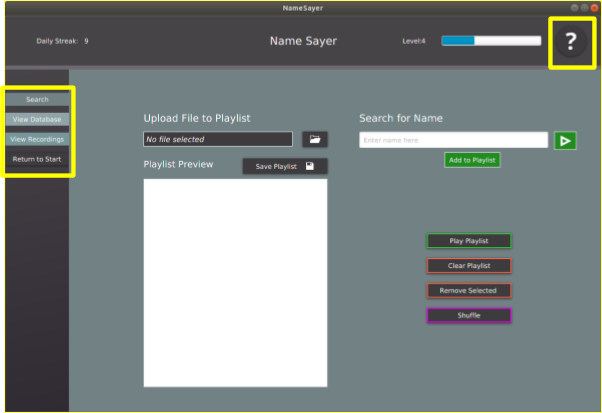
\includegraphics[width=\linewidth]{mainpane.png}
	\caption{Main Pane}
\end{figure}
The main pane consists of a header, sidebar and main body.
\\


The help button on the right takes you to this manual, if the manual is not located in the same directory as the jar file or you do not have an application for opening pdf files installed, an error message will appear.
\\


The options in the sidebar determine what is shown on the main body of the main pane.
\\


The main body defaults to the search pane which you can also navigate to by selecting the “Search” option on the sidebar. See Search Pane section for more info.
\\


The “View Database” option takes you to the view database pane. See the View Database section for more info.
\\


The “View Recordings” option takes you to the view recordings pane. See the View Recordings section for more info.
\\


You can also return to the start menu using the “Return to Start” button.
\newpage
\subsection{Daily Streak}
\begin{figure}[!h]
	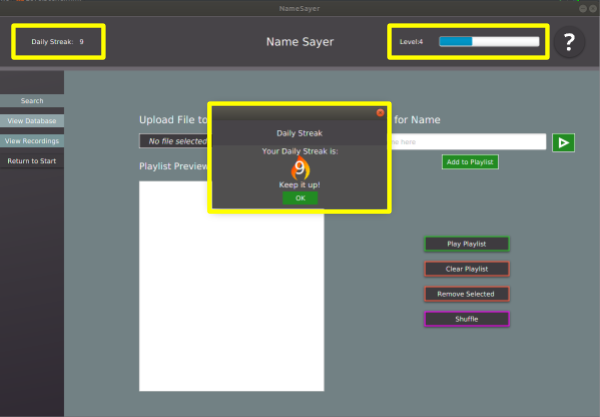
\includegraphics[width=\linewidth]{streaks.png}
	\caption{Daily Streak and Levelling System}
\end{figure}
The first time you enter the main pane, your daily streaks will be shown in a pop-up window.
\\


Your daily streak counts the number of successive days you have logged in to the NameSayer application. If you don’t log in for one day, you will lose your streak. 
\\


Your daily streak is always displayed in the header of the main pane.
\subsection{Levelling System}
In the header of the main pane you will see your experience level in the top right.
\\


Initially you start at level 1. To increase your level you need to practise names by recording and comparing yourself to the database recordings. 
\\

The amount of experience you gain is dependent on how well you pronounced the recording. See the ‘Comparing your recording with the database’ section for more information. 

\section{Search Pane} 
\subsection{Fusing/Searching recordings of first and family names together}
\begin{figure}[!h]
	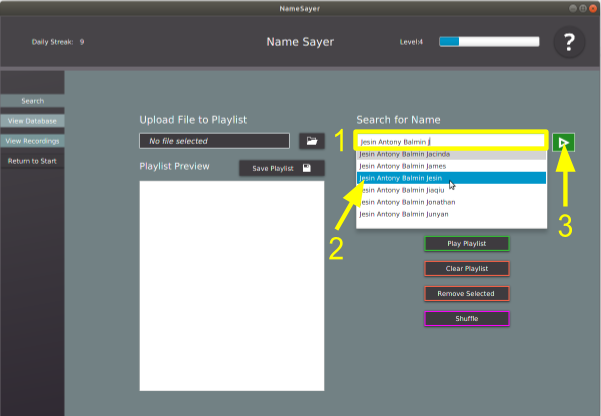
\includegraphics[width=\linewidth]{search.png}
	\caption{Fusing/Searching Names}
\end{figure}
\begin{enumerate}[label=\textbf{\arabic*}]
	\item To specify multiple names to fuse together type your desired name in the "Search for Name" text field. Your names can be of the form:
	
	
	\textit{$\langle First Name(s)\rangle$...$\langle Middle Name(s)\rangle$...$\langle Last Name(s)\rangle$}
	
	
	
	You can have as many first, middle and last names as you want. Either a space or hyphen can separate each name.

	\item While typing, you will receive suggestions in a drop-down box related to what you are typing. This will help you search for the names you are looking for.
	
	You can use the UP and DOWN arrow keys to navigate through the suggestions. Press ENTER on the suggestion you want, and it will autocomplete your name.

	\item When you have completed your name, press the button with the "Play" symbol. This will take you to the play scene where you can playback and practise the name. 

	Alternatively, you can press the "Add to Playlist" button or simply press the ENTER key in the text field and the name will be added to the playlist.

\end{enumerate}
\subsection{Uploading Text File with List of Names}
\begin{figure}[!h]
	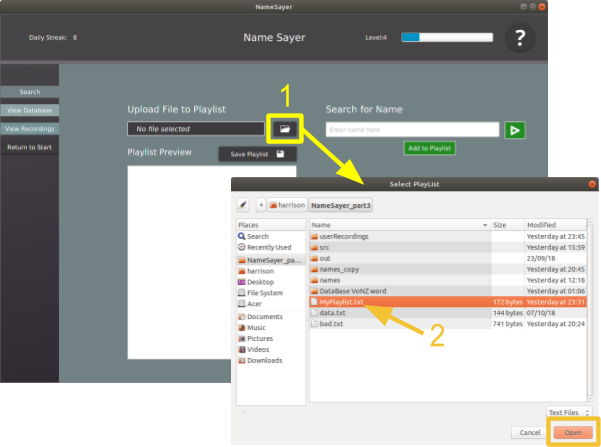
\includegraphics[width=\linewidth]{upload.png}
	\caption{Uploading a Text File}
\end{figure}

\begin{enumerate}[label=\textbf{\arabic*}]
	\item To upload your own text file to practise, press the button with the "Folder" symbol.
	
	\item A new window will open, double-click the text file containing the names you wish to upload or select it and press the “Open” button. Note that the text file should have the following format:
	\begin{figure}[!h]
		\centering
		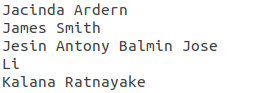
\includegraphics[width=7cm]{textfile.png}
		\caption{Example of Text File Format}
	\end{figure}
	\\
	This means each name should occupy its own line in the file.

	
	\item After selecting the file you will have to wait for it to load in. It will then appear in the playlist as seen in the next section.
	
\end{enumerate}
\newpage
\subsection{Using a Playlist}
\begin{figure}[!h]
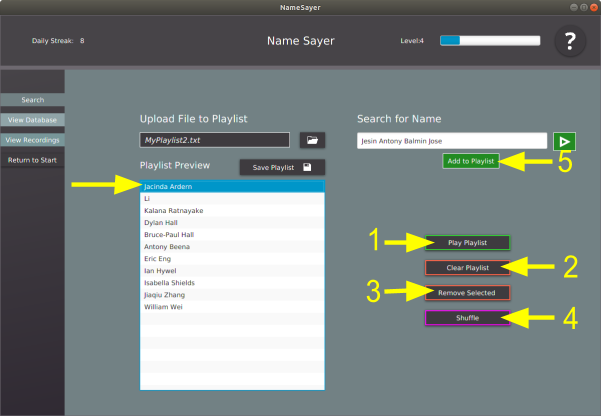
\includegraphics[width=\linewidth]{playlist.png}
\caption{Using a Playlist}
\end{figure}
\begin{enumerate}[label=\textbf{\arabic*}]
	\item Press the "Play Playlist" button to move to the play scene to practise and iterate through all names in the playlist.
	
	\item Press the "Clear Playlist" button to remove all names from the playlist and start a new playlist.
	
	\item Press the "Remove Selected" button to remove all selected names from the playlist. A selected name is highlighted in blue, multiple names or a single name can be highlighted blue by clicking on them.
	
	\item Press the "Shuffle" button to randomise the order in which the playlist is arranged. The order in which they appear in the playlist is the order in which they will be practised in the play scene.
	
	\item Press the "Add to Playlist" button to add the name that is currently in the "Search for Name" text field.
\end{enumerate}
\newpage

\subsection{Saving a Playlist}
\begin{figure}[!h]
	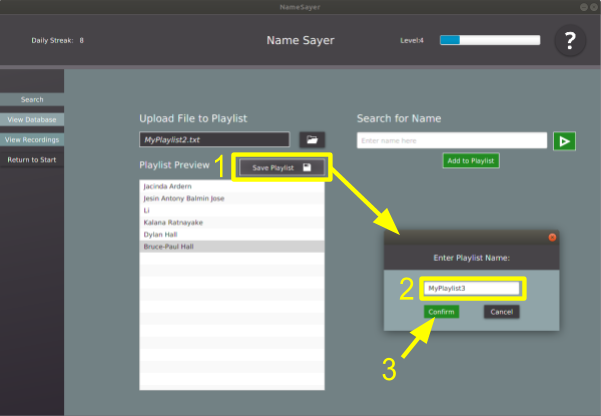
\includegraphics[width=\linewidth]{saving.png}
	\caption{Saving a Playlist}
\end{figure}
After adding and removing some names from a playlist, you may decide you want to keep it for later use. Instead of having to leave the application and manually write the names to a text file you can save the playlist very quickly from the application. This creates a new text file for you so you can upload and reuse it next time. 
\\


How to save a playlist:


\begin{enumerate}[label=\textbf{\arabic*}]
	\item Once you are happy with the names that are currently displayed in the playlist, press the "Save Playlist" button. 
	
	\item A new window is opened. In the text field enter the name of the text file you wish to save this playlist as. 
	
	**Note that any existing text files with the same name will be overwritten. 
	
	\item Press the "Confirm" button, your playlist will be saved, and the save window will close.
\end{enumerate}
\newpage

\section{View Database}
\begin{figure}[!h]
	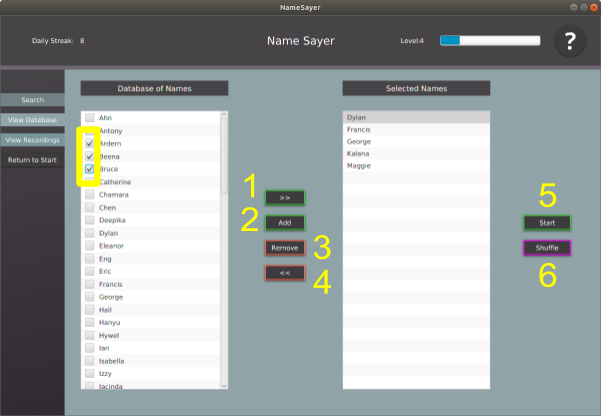
\includegraphics[width=\linewidth]{viewdb.png}
	\caption{Viewing the Database}
\end{figure}
The view database pane allows you to select names from the database and practise them.
\\ 

The list of names in the database is displayed in the tree on the left under the heading “Database of Names”. The list of selected names is displayed in a list on the right under the heading “Selected Names”.

\begin{enumerate}[label=\textbf{\arabic*}]
	\item To practise names, click the checkbox next to the names you wish to practise and then click the add button.
	
	\item To add all names in the database to the selected list, click the “>>” button. 
	
	\item To remove names from the selected list, click on the name in the selected list and click the remove button.
	
	\item To clear all names from the selected list click the “<<” button.
	
	\item If you want to randomise the order of names in the selected list, click the shuffle button on the right.
	
	\item When you are happy with the selected list, pressing start will take you to the play scene where you can begin practising.
\end{enumerate}
\newpage

\section{View Attempts/Recordings}
\begin{figure}[!h]
	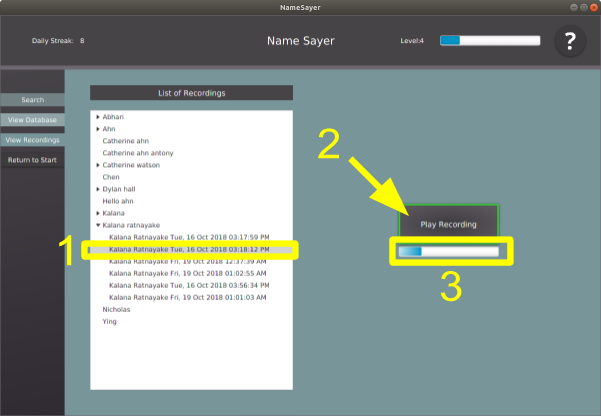
\includegraphics[width=\linewidth]{viewrec.png}
	\caption{Viewing Attempts/Recordings}
\end{figure}
The view recordings pane allows you to listen to and compare your previous attempts/recordings.
\\


The recordings are displayed in a tree under the heading “List of Recordings”.
\\


The recordings are identified by the name that is recorded and the date and time when it was recorded, allowing you to differentiate between the different versions.

\begin{enumerate}[label=\textbf{\arabic*}]
	\item To play a recording, select the recording in the tree.
	
	\item Press the “Play Recording” button on the right.
	
	\item When the recording begins, the progress bar beneath the “Play Recording” button will also begin, showing you that the recording is playing.
\end{enumerate}
\newpage

\section{Play Scene}
\begin{figure}[!h]
	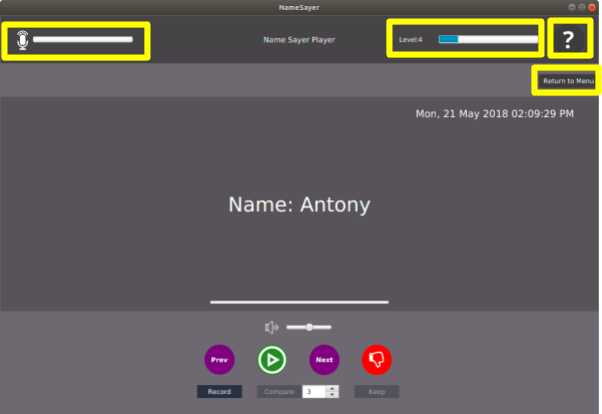
\includegraphics[width=\linewidth]{play.png}
	\caption{Play Scene}
\end{figure}
The play scene allows you to practise saying the names by listening to the recording from the database, creating your own recording and then comparing your recording with the recording in the database.
\\


The header of the play scene also shows the users mic level, experience level and the help button which links to this manual.
\\


You can return to the main pane at any time by pressing the “Return to Menu” button on the top right.

\newpage

\subsection{Listening to Recordings}
\begin{figure}[!h]
	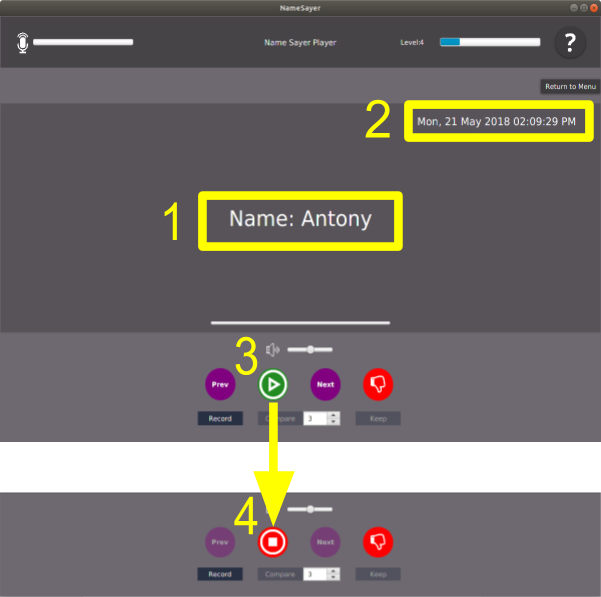
\includegraphics[width=\linewidth]{listen.png}
	\caption{Playing Recordings}
\end{figure}
\begin{enumerate}[label=\textbf{\arabic*}]
	\item The name of the current recording is displayed in the centre of the scene.
	
	\item The date when it was recorded is displayed on the top right.
	
	\item To play the current name, click the green play button. 
	
	\item When the recording is playing, the play button turns into a stop button. To stop the playback, click the stop button.
	
\end{enumerate}
When the recording has finished playing, or the stop button is pressed, the stop button turns back into the play button.
\\


You can press the play button again to listen to the recording as many times as you want.

\subsection{Cycling through the Playlist}
\begin{figure}[!h]
	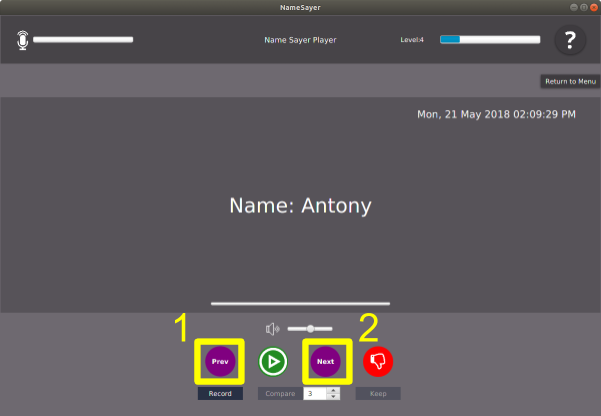
\includegraphics[width=\linewidth]{cycling.png}
	\caption{Cycling through Recordings}
\end{figure}
You can cycle through the list of names you selected either from the search pane or view database pane using the next and previous buttons.
\begin{enumerate}[label=\textbf{\arabic*}]
	\item The “Prev” button changes the displayed recording to the previous recording in the list.
	
	The “Prev” button starts disabled and only becomes enabled if the current recording is not the first in the list.
	
	\item The “Next” button changes the displayed recording to the next recording in the list.
	
	The “Next” button becomes disabled once you reach the end of your list.
	
\end{enumerate}
\newpage

\subsection{Rating the Quality of the Recording}
\begin{figure}[!h]
	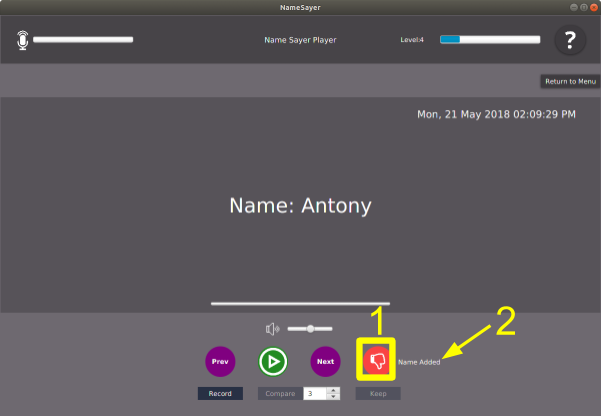
\includegraphics[width=\linewidth]{rating.png}
	\caption{Rating the Recordings}
\end{figure}
\begin{enumerate}[label=\textbf{\arabic*}]
	\item The “Prev” button changes the displayed recording to the previous recording in the list.
	
	The “Prev” button starts disabled and only becomes enabled if the current recording is not the first in the list.
	
	\item Pressing the bad button displays a message notifying you that the recording has been marked as bad.
\end{enumerate}
All recordings marked as bad are added to the 'bad.txt' file in the current working directory which keeps a record of the bad recordings so that an admin can decide what to do with them later.
\newpage

\subsection{Creating your own Recording}
\begin{figure}[!h]
	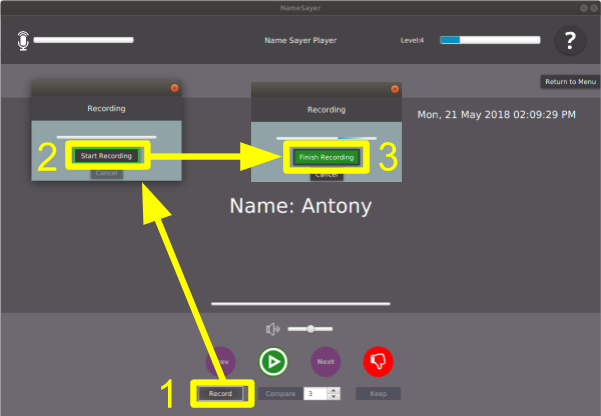
\includegraphics[width=\linewidth]{record.png}
	\caption{Creating a Recording}
\end{figure}
\begin{enumerate}[label=\textbf{\arabic*}]
	\item If you want to create your own recording of the current name, click the record button and a recording window will show up.
	
	\item When you are ready to begin, recording press the “Start Recording” button.
	
	
	
	The progress bar will start when you are recording, and the “Start Recording” button will be replaced with a “Finish Recording” button.
	
	\item When you have finished recording press the “Finish Recording”. This will take you back to the play scene.
	
\end{enumerate}
Note that the maximum recording time allowed is 15 seconds.
\\


If you want to return to the play scene without finishing a recording, press the “Cancel” button.

\newpage

\subsection{Comparing your recording with the database}
\begin{figure}[!h]
	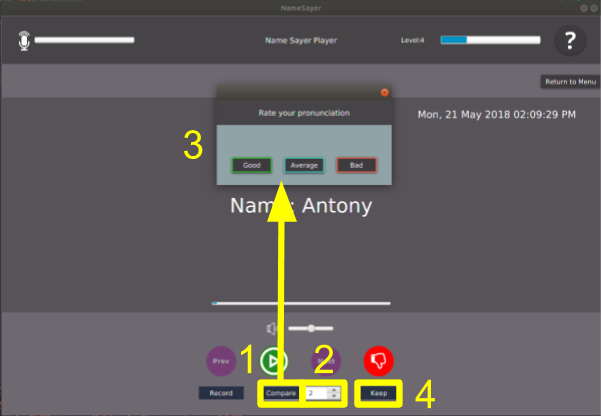
\includegraphics[width=\linewidth]{compare.png}
	\caption{Comparing your Recording}
\end{figure}
The compare functionality becomes enabled after you have created your own recording of the current name.
\begin{enumerate}[label=\textbf{\arabic*}]
	\item Click the “Compare” button to play your recording followed by the database recording, 3 times.
	
	\item You can choose the number of times (between 1 and 10) the recordings loop by adjusting the spinner next to the “Compare” button.
	
	\item After comparing the first time, a window will appear asking if you thought your recording was good, average, or bad. 
	
	How you performed will influence how much experience you receive.
	
	\item If you want to keep your recording, simply press the “Keep” button next to compare, which should be enabled after you created a recording.
	
	When you press the “Keep” button a message will appear notifying you the recording has been saved and can be accessed in the View Recordings pane.
\end{enumerate}
\newpage

\section{Missing Names}
\begin{figure}[!h]
	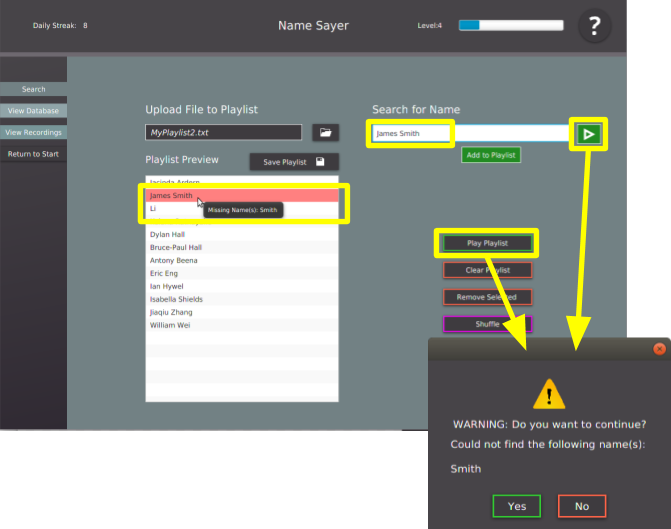
\includegraphics[width=\linewidth]{missing.png}
	\caption{Missing Names in the Search Pane}
\end{figure}
When a name recording is missing from the selected database, there are different ways to deal with them.
\begin{itemize}
	\item When you have entered a missing name and the “Play” symbol button is pressed, you will be notified of a warning which shows you the names that are not in the database. 
	
	\item When a name that contains a recording that is not in the database is added to the playlist, it will be highlighted red in the playlist view.
	
	\item To find out which name recordings are missing from the name, simply hover over the entry in the playlist and a helpful tooltip will appear.
	
	\item In either case, you can choose to remove/ignore the name. Or you can continue to the play scene to practise with the found audio and without the missing audio.
\end{itemize}

\newpage
\end{document}